\documentclass[12pt,a4paper]{article}

\usepackage{graphicx}% Include figure files
\usepackage{dcolumn}% Align table columns on decimal point
\usepackage{bm}% bold math
%\usepackage{hyperref}% add hypertext capabilities
%\usepackage[mathlines]{lineno}% Enable numbering of text and display math
%\linenumbers\relax % Commence numbering lines

%\usepackage[showframe,%Uncomment any one of the following lines to test 
%%scale=0.7, marginratio={1:1, 2:3}, ignoreall,% default settings
%%text={7in,10in},centering,
%%margin=1.5in,
%%total={6.5in,8.75in}, top=1.2in, left=0.9in, includefoot,
%%height=10in,a5paper,hmargin={3cm,0.8in},
%]{geometry}

\usepackage{multicol}%Para hacer varias columnas
\usepackage{multicol,caption}
\usepackage{multirow}
\usepackage{cancel}
\usepackage{hyperref}
\hypersetup{
    colorlinks=true,
    linkcolor=blue,
    filecolor=magenta,      
    urlcolor=cyan,
}

\setlength{\topmargin}{-1.0in}
\setlength{\oddsidemargin}{-0.3pc}
\setlength{\evensidemargin}{-0.3pc}
\setlength{\textwidth}{6.75in}
\setlength{\textheight}{9.5in}
\setlength{\parskip}{0.5pc}

\usepackage[utf8]{inputenc}
\usepackage{expl3,xparse,xcoffins,titling,kantlipsum}
\usepackage{graphicx}
\usepackage{xcolor} 
\usepackage{siunitx}
\usepackage{nopageno}
\usepackage{lettrine}
\usepackage{caption}
\renewcommand{\figurename}{Figura}
\usepackage{float}
\renewcommand\refname{Bibliograf\'ia}
\usepackage{amssymb}
\usepackage{amsmath}
\usepackage[rightcaption]{sidecap}
\usepackage[spanish]{babel}

\providecommand{\abs}[1]{\lvert#1\rvert}
\providecommand{\norm}[1]{\lVert#1\rVert}
\newcommand{\dbar}{\mathchar'26\mkern-12mu d}

% CABECERA Y PIE DE PÁGINA %%%%%
\usepackage{fancyhdr}
\pagestyle{fancy}
\fancyhf{}

\begin{document}

Macías Márquez Misael Iván


\textbf{PRIMERA PARTE}

\begin{enumerate}



%%%1%%%



\item Si la capacidad calorífica del agua fuese menor, entonces:¿Sería más probable o menos probable que un lago se congelara en invierno? Explica tu respuesta. Por último : ¿A qué se debe que los lagos y estanques se congelen de arriba hacia abajo y no de abajo hacia arriba?

\textbf{Sol:}

Pues ya que la capacidad calorífica nos dice en su forma diferencial que tanto calor necesita ser absorbido por cierta cantidad de materia para que esta se caliente un intervalo de temperatura, entonces si la disminuimos se requerirá una cantidad menor de calor para aumentar y por ende disminuir la temperatura ,por lo tanto, sí sería más probable que un lago se congelara en invierno.

Como vimos en clase, la densidad del agua a presión constante disminuye conforme la temperatura lo hace, excepto en un cierto rango de valores para la temperatura ($0^{\circ}C$ a $4^{\circ}C$ ), en este intervalo la densidad aumenta junto con la temperatura, gracias a esta diferencia de densidades, cuando un lago/estanque se enfría, lo hace rotando el agua en la superficie (más fría) con el agua en el interior (más caliente), esto sucede hasta llegar a los $4^{\circ}C$ donde al disminuir la densidad al mismo tiempo que la temperatura, el movimiento de rotación se concluye provocando una diferencia de temperatura en una capa de la superficie que al llegar a los $0^{\circ}C$ se congela mientras que el resto del agua se mantiene relativamente constante en su temperatura, por lo tanto para que el agua de un lago/estanque se congele de abajo hacia arriba, se debería mantener la tendencia de valores mayores a $4^{\circ}C$ de la densidad del agua con la temperatura. 




%%%2%%%



\item Islandia (que en islandés significa Tierra del Hielo) fue llamada así para desalentar a los posibles conquistadores de imperios en expansión. Sin embargo, Islandia NO está cubierta completamente de hielo como Groenlandia o Siberia a pesar de estar muy cercana al circulo ártico. La temperatura invernal promedio de Islandia es considerablemente mayor a las de ciertas regiones del este de Groenlandia y el centro de Siberia ubicadas a la misma latitud. ¿A qué se debe esto?

\textbf{Sol:}

Después de pensarlo mucho, no se me ocurrió nada así que investigue sobre el país y al parecer esto se debe a la corriente del Golfo, esta corriente se origina en el Golfo de México llevando agua caliente hacia el norte entre Europa y Groenlandia, esta corriente al ser menos densa (por la temperatura y cuestiones de salinidad) pasa cerca de la superficie pero al llegar a su destino esta se enfría y se saliniza  por lo que se va a la parte inferior de océano y regresa al golfo a calentarse (dato triste: esta corriente está perdiendo fuerza gracias al derretimiento de los glaciares). Así que esta corriente es la responsable del clima relativamente cálido sobre las regiones cercanas a la misma ya que funciona como un refrigerador invertido llevando el calor del trópico de Cáncer al círculo polar Ártico.



\newpage
%%%3%%% 



\item ¿Qué le ocurre a la energía interna de un sistema cuando sobre él se realiza trabajo?, ¿Qué le sucede a la temperatura del sistema cuando sobre él se realiza trabajo? Por último: cuando inflas un neumático de bicicleta con una bomba, el cilindro de la bomba se calienta. Da dos razones de este fenómeno.

\textbf{Sol:}

Por la primera ley, sabemos que $\dbar Q  = dU - \dbar W$ así que se tiene un proceso adiabático, la energía interna tendrá el mismo cambio del trabajo suministrado, si es isotérmico, como la energía interna depende del cambio de temperatura entonces la energía interna se mantendrá constante.

La temperatura sobre el sistema al que se le suministra trabajo puede ser calentado o bien no tener ningún cambio sobre su temperatura.


El cilindro de la bomba se calienta en parte por la fricción del pistón y también debido a que el gas que se encuentra adentro se comprime antes de salir al neumático por lo que se le suministra calor y aumenta su temperatura que al estar en contacto con el cilindro suponiendo que este se encuentre a una menor temperatura que la del gas, recibe cierto calor del gas.
    
\end{enumerate}


\textbf{SEGUNDA PARTE}

\begin{enumerate}
    \item Escribe la ecuación de estado para un gas de van der Waals. Posteriormente analiza para el polinomio de grado 3 en el volumen lo que sucede para temperaturas mayores y menores a la crítica, tal como lo discutimos en clase. Apóyate en este desarrollo en un diagrama $P-V$ donde muestres las isotermas. Posteriormente encuentra la ecuación de parámetros reducidos:
    
    \begin{equation*}
        \left(\pi + \frac{3}{\phi^2}\right) (3\phi -1) = 8 \tau
    \end{equation*}
    
    Recuerda que en el punto crítico se satisface:
    
    \begin{equation*}
        \left(\frac{\partial p}{\partial v}\right)_{\theta = \theta_C} =0\hspace{4cm} \left(\frac{\partial^2 p}{\partial v^2}\right)_{\theta = \theta_C} =0
    \end{equation*}
    
    \textbf{Sol:}
    
    La ecuación de estado de Van der Waals es
    
    \begin{equation}
        p = \frac{R \theta}{v-b} - \frac{a}{v^2}
    \end{equation}
    
    \begin{figure}[h!]
        \centering
        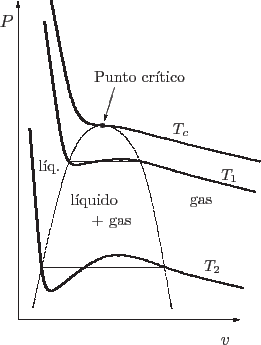
\includegraphics[scale=0.6]{img823.png}
        \caption{https://www.famaf.unc.edu.ar/~gcas/termo1/clases/node64.html}
    \end{figure}
    
    para un mol, esta ecuación puede escribirse como
    
    \begin{equation}
        v^3 - \left(\frac{R\theta}{p} + b\right) v^2 + \frac{a}{p} v - \frac{ab}{p} = 0
    \end{equation}
    
    \newpage
    
    Pues para temperaturas mayores a la crítica no se tienen puras raíces reales (a lo mucho una raíz real ya que las complejas vienen en pares y porque tenemos un polinomio de grado 3) dándonos la ecuación del gas ideal, para temperaturas menores a la crítica se tienen raíces reales.
    
    Como (2) es un polinomio de grado 3, ya que en el punto crítico se tiene una triple raíz (como se ve en la figura 1), entonces podemos escribir a (2) como
    
    \begin{equation}
        (v - v_c)^3 = 0 \hspace{1cm} \rightarrow \hspace{1cm} v^3 - 3v_c v^3 + 3v_{c}^{2}v - v_{c}^{3} = 0
    \end{equation}
    
    y como (3) debe ser igual a (2), entonces
    
    \begin{equation}
        3v_c = \frac{RT_c}{p_c} + b \hspace{1cm} 3v_{c}^{2} =\frac{a}{p_c} \hspace{1cm} v_{c}^{3} = \frac{ab}{p_c}
    \end{equation}
    
    despejando una $v_c$ de (4.3) y sustituyendo en (4.2) llegamos a que $v_c = 3b$, sustituyendo lo anterior en (4.3) obtenemos $p_c = \frac{a}{27 b^2}$,y despejando $\theta_c$ de (4.1) y sustituyendo los 2 resultados obtenidos anteriormente se tiene que $\theta_c = \frac{8a}{27Rb}$, por lo tanto
    
    \begin{equation}
        \theta_c = \frac{8a}{27Rb} \hspace{1cm} p_c = \frac{a}{27b^2} \hspace{1cm} v_c = 3b
    \end{equation}
    
    ahora despejando $p_c$ de (5.3), $b = \frac{v_c}{3}$, despejando $a$ de (5.2) y sustituyendo $b$, $a = 3p_c v_{c}^{2}$ y sustituyendo los resultados anteriores en (5.1), $\theta_c = \frac{8p_c v_c}{3R}$, y así
    
    \begin{equation}
        \theta_c = \frac{8p_c v_c}{3R} \hspace{1cm} a = 3p_c v_{c}^{2} \hspace{1cm} b = \frac{v_c}{3}
    \end{equation}
    
    y sustituyendo todo esto en (1)
    
    \begin{equation}
         \frac{p}{p_c} = 8 \frac{\theta}{\theta_c(3\frac{v}{v_c}-1)} - \frac{3}{(\frac{v}{v_c})^2}
    \end{equation}
    
    Sea $\pi = \frac{p}{p_c}$, $\phi = \frac{v}{v_c}$ y $\tau = \frac{\theta}{\theta_c}$, entonces (7) toma la forma de
    
    \begin{equation}
        \pi = 8\tau \frac{1}{3\phi - 1} - \frac{3}{\omega^2} \hspace{1cm} \rightarrow \hspace{1cm} 8 \tau = \left(\pi +\frac{3}{\phi^2}\right)(3\phi -1)
    \end{equation}
    
    \begin{enumerate}
        \item Explica con tus propias palabras que significan los términos $\mathbf{a}$ y $\mathbf{b}$ en la ecuación de Van der Waals.
        
        \textbf{Sol:}
        
        El parámetro $\mathbf{b}$ en la ecuación de Van der Waals describe el espacio que ocupan las moléculas del gas en estudio, suponiendo que este solo tenga un tipo de molécula componente, caso contrario, creo que puede significar el volumen promedio ocupado por las moléculas del gas, este parámetro es necesario ya que en un gas real las moléculas ocupan un espacio considerable del volumen que los contiene por lo que el volumen disponible se reduce.
        
        El parámetro $\mathbf{a}$ sirve para compensar la diferencia de presión debido a las interacciones de las propias moléculas del gas algo que en un gas ideal no es necesario ya que las moléculas están lo suficientemente espaciadas como para sentir que están solas.
        
        
        \item ¿Por qué esta ecuación predice cualitativamente la transición líquido-gas?
        
        \textbf{Sol:}
        
        Esto es gracias a que para valores de la temperatura menores a la crítica, se tiene que para cierto volumen existen 2 posibles volúmenes que pueden interpretarse como los volúmenes del gas en estado líquido y gaseoso.
        
        
        
        
        \item ¿Qué significa tener una ecuación de parámetros reducidos?, ¿Qué información física proporciona?
        
        \textbf{Sol:}
        
        La ecuación de parámetros reducidos al no tener los parámetros $\mathbf{a}$ y $\mathbf{b}$, funciona para cualquier gas sin importar sus cualidades y al ser adimensional está ecuación es exactamente igual para cualquier gas, es decir, se puede describir el comportamiento de cualquier gas sin importar como sea con (8).
        
        
        
        
        \item Utilizando la ecuación de estado de Van der Waals, muestra que el coeficiente de compresibilidad isotérmica $\kappa_{T}$ viene dado por:
        
        
        \begin{equation*}
            \kappa_{\theta} = \frac{\frac{v-b}{v}}{p - \frac{a(v-2b)}{v^3}} = \frac{(v-b)^2}{R v} \frac{1}{\theta - \frac{2a(v-b)^2}{Rv^3}}
        \end{equation*}
        
        
        \textbf{Sol:}
        
        Primero multipliquemos (2) por $p$
        
        \begin{equation}
          f=   pv^3 - (R\theta + bp) v^2 + av - ab = 0
        \end{equation}
        
        ahora despejemos a $p$
        
        \begin{equation}
            p = \frac{R\theta v^2 - a(v-b)}{(v-b)v^2}
        \end{equation}
        
        entonces derivando (9)
        
        \begin{equation}
        \left(\frac{\partial f}{\partial v}\right) dv + \left(\frac{\partial f}{\partial p}\right) dp + \left(\frac{\partial f}{\partial \theta}\right) d\theta = (3v^2p - 2pbv-2r\theta) dv + (v^3 - bv^2)dp - Rv^2 d\theta =0
        \end{equation}
        
        y entonces
        
        \begin{equation}
            \kappa_{\theta} = -\frac{1}{v} \left(\frac{\partial v}{\partial p}\right)_{\theta} = \frac{v^2 -bv}{3pv^2 - 2vbp+2vR\theta + a}
        \end{equation}
        
        y sustituyendo (10) en (12)
        
        \begin{equation}
            \kappa_{\theta} = \frac{v^2 (v-b)^2}{R\theta v^3 - 2a(v-b)^2/v} = \frac{(v-b)^2}{R v} \frac{1}{\theta - \frac{2a(v-b)^2}{Rv^3}}
        \end{equation}
        
        
        
        \item Demuestra que el coeficiente de expansión isobárico viene dado por :
        
        \begin{equation*}
            \beta =\frac{\frac{v-b}{v}}{\theta - \frac{2a(v-b)^2}{Rv^3}} 
        \end{equation*}
    
        \textbf{Sol:}
        
        Usando de nuevo a (11)
        
        \begin{equation}
            \beta = \frac{1}{V} \left(\frac{\partial v}{\partial \theta}\right)_{p} = \frac{Rv}{(3v-2b)vp-2R\theta v + a}
        \end{equation}
        
        y sustituyendo (10)
        
        \begin{equation}
            \beta = \frac{Rv^2 (v-b)}{R\theta v^3 - 2a (v-b)^2} = \frac{\frac{v-b}{v}}{\theta - \frac{2a(v-b)^2}{Rv^3}} 
        \end{equation}
        
    \end{enumerate}
    
    
    
%%%2%%%
    
    
    
    \item Dibuja en un diagrama $P- V$ el ciclo de un motor Diesel cuando la sustancia operante es un gas ideal. Deberás explicar en qué consisten todos los procesos, es decir, deberás explicar lo que sucede al gas durante todas las carreras que componen el ciclo. Después deberá elaborar una tabla $P - V - \theta$ para cada punto del ciclo. Por último, analizando cada proceso por separado, calcula la eficiencia total dada por:
    
    \begin{equation*}
        \eta = 1 - \frac{1}{\gamma} \left[\frac{\left(\frac{1}{r_E}\right)^{\gamma} - \left(\frac{1}{r_C}\right)^{\gamma}}{\frac{1}{r_E} - \frac{1}{r_C}}\right]
    \end{equation*}
    
    Donde:
    
    \begin{equation*}
        r_E = \frac{V_1}{V_3} \hspace{4cm} r_C = \frac{V_1}{V_2}
    \end{equation*}
    
    
    \textbf{Sol:}
    
    Supongamos que tenemos un mol ($n=1$)
    
    \begin{figure}[h!]
        \centering
        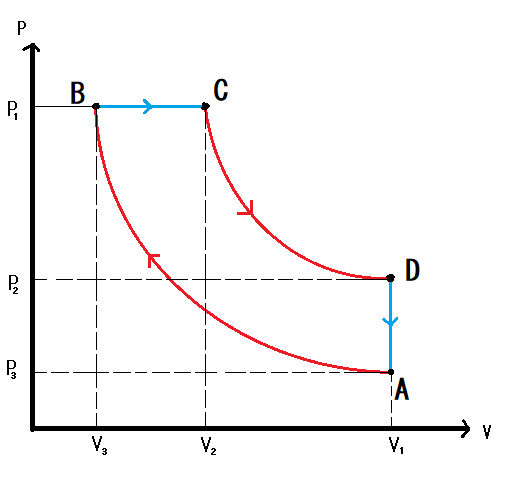
\includegraphics[scale=0.8]{1.png}
    \end{figure}
    
    En el proceso $AB$ el gas sufre una compresión de manera adiabática, en $BC$ se tiene una inyección de combustible  que al hacer combustión aumenta el volumen y la temperatura, en $CD$ tenemos otro proceso adiabático pero esta vez es una expansión y por último en $DA$ la presión del gas disminuye mientras el volumen queda constante por lo que hay una disminución de la temperatura.
    
    Como tenemos un mol de gas ideal ($PV = R\theta$)
    
    \begin{table}[h!]
        \centering
        \begin{tabular}{|l|c|c|c|}
        \hline
           & $P$ & $V$ & $\theta$ \\ \hline
            A & $P_3$ & $V_1$ & $\frac{P_3 V_1}{R}$\\
            B & $P_1$ & $V_3$ & $\frac{P_1 V_3}{R}$\\
            C & $P_1$ & $V_2$ & $\frac{P_1 V_2}{R}$\\
            D & $P_2$ & $V_1$ & $\frac{P_2 V_1}{R}$ \\ \hline
        \end{tabular}
    \end{table}
\end{enumerate}

Ahora obtengamos la eficiencia, como los procesos $AB$ y $CD$ son adiabáticos, la trasferencia de calor del ciclo se debe dar en los procesos $BC$ y $DA$, como estos procesos son isocórico e isobárico y como el aumento de temperatura se da en $BC$, el calor de cada proceso es

\begin{equation}
  Q_{H} = \frac{P_1 C_{P}}{R} ( V_3 - V_2)  
\end{equation}

\begin{equation}
    Q_{C} = \frac{V_1 C_V}{R} (P_3 - P_2)
\end{equation}

entonces la eficiencia de este motor es

\begin{equation}
    \eta = 1 - \frac{Q_C}{Q_H} = 1 - \frac{\frac{V_1 C_V}{\cancel{R}} (P_3 - P_2)}{ \frac{P_1 C_{P}}{\cancel{R}} ( V_3 - V_2)} = 1 -\frac{1}{\gamma} \frac{V_1(P_3 - P_2)}{P_1(V_3 - V_2)}
\end{equation}

donde $\gamma = \frac{C_P}{C_V}$, y multiplicando (18) por $P_1 V_1 /P_1 V_1$

\begin{equation}
    \eta = 1 -\frac{1}{\gamma} \frac{(\frac{P_3}{P_1} - \frac{P_2}{P_1})}{(\frac{V_3}{V_1} - \frac{V_2}{V_1})} = 1 - \frac{1}{\gamma} \frac{(\frac{P_3}{P_1} - \frac{P_2}{P_1})}{\frac{1}{r_E} - \frac{1}{r_C}}
\end{equation}

pero como $AB$ y $CD$ son adiabáticos, entonces se tiene $P_3 V_{1}^{\gamma}= P_1 V_{3}^{\gamma}$ y $P_1 V_{2}^{\gamma} = P_{2} V_{1}^{\gamma}$ o bien $\frac{P_2}{P_1} = \frac{V_{2}^{\gamma}}{V_{1}^{\gamma}} =  (\frac{1}{r_E}) ^{\gamma}$ y $\frac{P_3}{P_1} = \frac{V_{3}^{\gamma}}{V_{1}^{\gamma}} = (\frac{1}{r_C})^{\gamma}$ que sustituyendo en (19)

\begin{equation*}
    \eta = 1 - \frac{1}{\gamma} \left[\frac{\left(\frac{1}{r_E}\right)^{\gamma} - \left(\frac{1}{r_C}\right)^{\gamma}}{\frac{1}{r_E} - \frac{1}{r_C}}\right]
\end{equation*}

\end{document}